% **************************************************************
% Hi! Edit this file for your presentation!
% **************************************************************

% ==================///==================///==================///
% ==================/// LATEX'S STUFF
% ==================///==================///==================///

\documentclass{beamer}
\usepackage{amsfonts,amsmath,oldgerm}
\usepackage{listings}
\usepackage{graphics,graphicx}
\usepackage{mdframed} 
\usetheme{_statale}
\usefonttheme[onlymath]{serif}

\lstdefinestyle{statalepython}{
    language=Python,
    backgroundcolor=\color{statalegray},
    basicstyle=\scriptsize\ttfamily,
    keywordstyle=\color{maincolor}\bfseries,
    stringstyle=\color{statalegreen},
    commentstyle=\color{stataledarkgreen}\itshape,
    numberstyle=\tiny\color{gray},
    numbers=none,
    numbersep=8pt,
    stepnumber=1,
    showstringspaces=false,
    breaklines=true,
    frame=single,
    tabsize=4,
    captionpos=b
}

\newcommand{\testcolor}[1]{\colorbox{#1}{\textcolor{#1}{test}}~\texttt{#1}}
\newcommand{\hrefcol}[2]{\textcolor{cyan}{\href{#1}{#2}}}
\titlebackground*{assets/background}

% ==================///==================///==================///
% ==================/// SPLASH PAGE
% ==================///==================///==================///

\title{Verifiche di compliance in ambienti Cloud}
\subtitle{Presentazione dell'elaborato finale}
\course{Laurea Triennale in Sicurezza dei Sistemi e delle Reti Informatiche}
\author{\href{mailto:niccolo.volonte@studenti.unimi.it}{Niccolò Volontè}}
\IDnumber{20642A}
\relatore{Prof. Marco Anisetti}
\correlatore{Dott. Antongiacomo Polimeno}
\date{16 luglio 2025}

% ==================///==================///==================///
% ==================///  START PRESENTATION
% ==================///==================///==================///

\begin{document}
\maketitle

\footlinecolor{maincolor}


% ==================///==================///==================///
% ==================/// BODY'S PRESENTATION
% ==================///==================///==================///

\begin{frame}{Introduzione e contesto normativo}
    \framesubtitle{Cloud, compliance e obiettivi}
    \begin{columns}
        \begin{column}{0.7\textwidth}
                \begin{itemize}
                    \item<1-> Crescita del Cloud Computing e della sua adozione
                    \item<3-> La \emph{compliance} nel cloud: ambiente dinamico rende difficile la verifica del profilo di sicurezza
                    \item<4-> \textbf{Standard di riferimento}:
                    \begin{itemize}
                        \item CIS AWS Foundations Benchmark
                        \item NIST SP 800-53
                    \end{itemize}
                    \item<5-> \textbf{Obiettivo:} \emph{sviluppare} \textbf{sonde} automatizzabili per verifiche di \textbf{compliance} su \textbf{AWS}, \emph{integrabili} nella piattaforma \textbf{Moon Cloud}
                \end{itemize}
        \end{column}
        \begin{column}{0.3\textwidth}
            \includegraphics<2->[width=\textwidth]{assets/statista.jpeg}
            \vspace{1em}
            \includegraphics<4->[width=\textwidth]{assets/cisnist.png}
        \end{column}
    \end{columns}
\end{frame}



\begin{frame}{Standard di riferimento}
    \framesubtitle{Esempio di controllo per \texttt{aws\_account}}
    \begin{mdframed}[backgroundcolor=statalegrey]
    \textbf{1.4 Ensure MFA is enabled for the 'root' user account (Automated)}
    \begin{itemize}
        \item \textbf{Profile Applicability:} Level 1
        \item \textbf{Description:} The 'root' user account is the most privileged user in an AWS account. Multi-factor Authentication (MFA) adds an extra layer of protection on top of a username and password. With MFA enabled, when a user signs in to an AWS website, they will be prompted for their username and password as well as for an authentication code from their AWS MFA device.
        \item \textbf{Rationale:} Enabling MFA provides increased security for console access as it requires the authenticating principal to possess a device that emits a time-sensitive key and have knowledge of a credential.
    \end{itemize} 
\end{mdframed}
\end{frame}

% \begin{frame}{Tecnologie utilizzate}
%     \framesubtitle{Linguaggi e strumenti}
%     \begin{columns}
%         \begin{column}<1->{0.4\textwidth}
%             \begin{itemize}
%                 \item \emph{Python} come linguaggio di programmazione
%                 \item \texttt{Boto3} per l'interazione con AWS
%                 \item \emph{Moon Cloud} come piattaforma di integrazione
%             \end{itemize}
%         \end{column}
%         \begin{column}<2->{0.6\textwidth}
%             \begin{colorblock}[black]{statalegrey}{Esempio di utilizzo di Boto3}
%                 \texttt{\textcolor{maincolor}{import} boto3}\\
%                 \texttt{client = boto3.\textcolor{maincolor}{client}(}\\
%                 \texttt{    \textcolor{statalegreen}{'sqs'},}\\
%                 \texttt{    region\_name=\textcolor{statalegreen}{'eu-central-1'},}\\
%                 \texttt{    aws\_access\_key\_id=\textcolor{statalegreen}{'YOUR\_ACCESS\_KEY'},}\\
%                 \texttt{    aws\_secret\_access\_key=\textcolor{statalegreen}{'YOUR\_SECRET\_KEY'}}\\
%                 \texttt{)}\\
%                 \texttt{response = client.\textcolor{maincolor}{list\_queues}()}\\
%             \end{colorblock}
%         \end{column}
%     \end{columns}
% \end{frame}

\begin{frame}{Analisi della documentazione}
    \framesubtitle{AWS Security Hub, Boto3 Account}
    \begin{columns}
        \begin{column}{0.5\textwidth}
            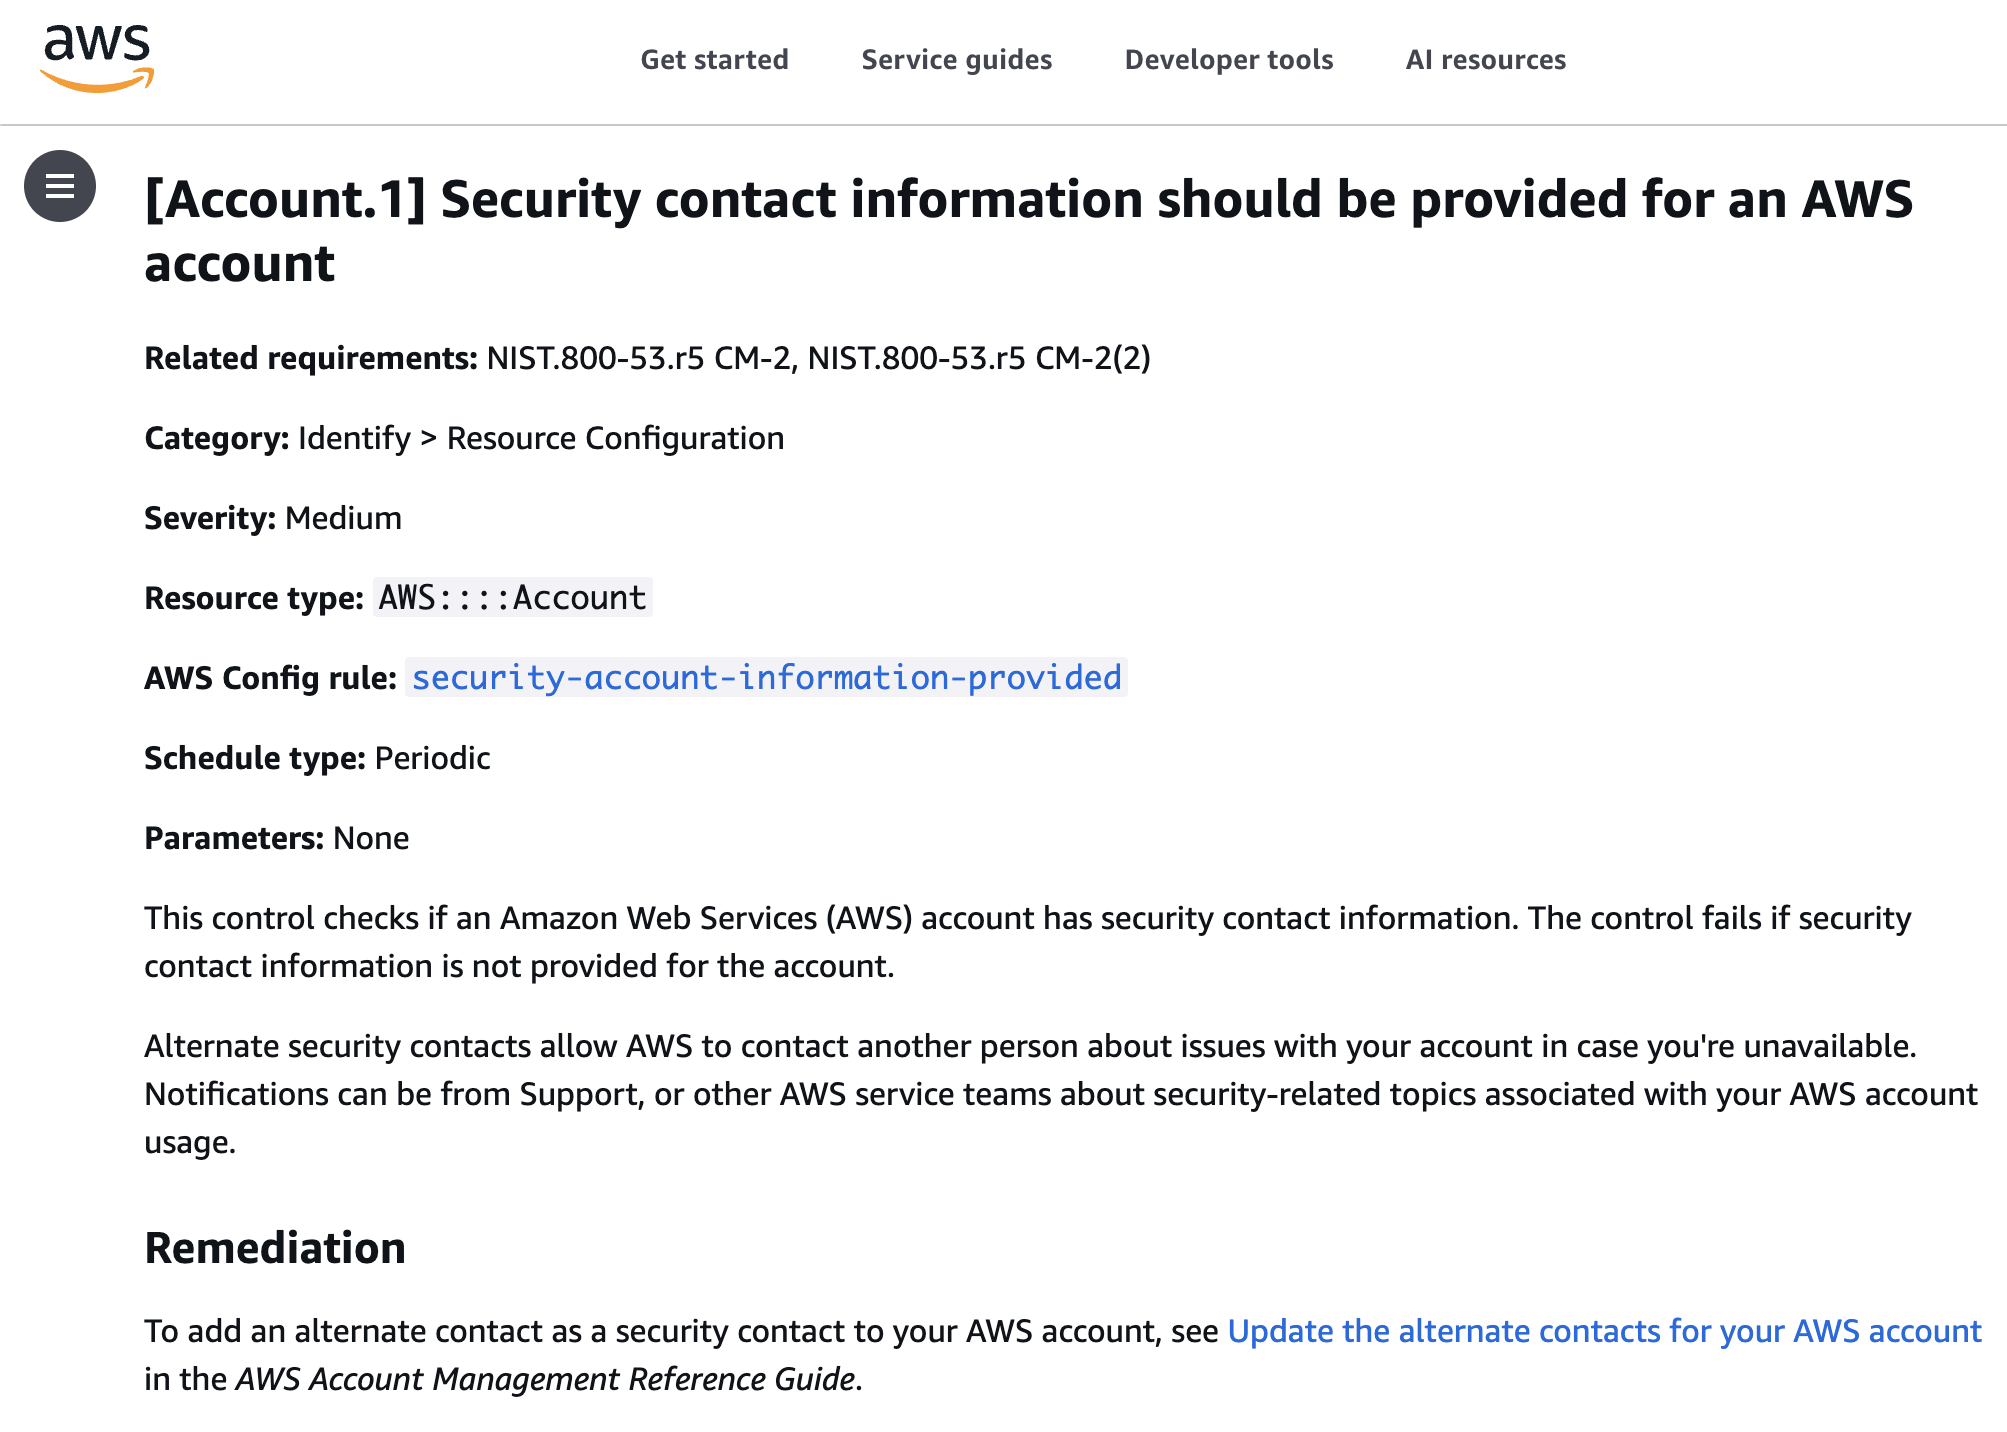
\includegraphics[width=\textwidth]{assets/sechubacc.png}
        \end{column}
        \begin{column}{0.5\textwidth}
            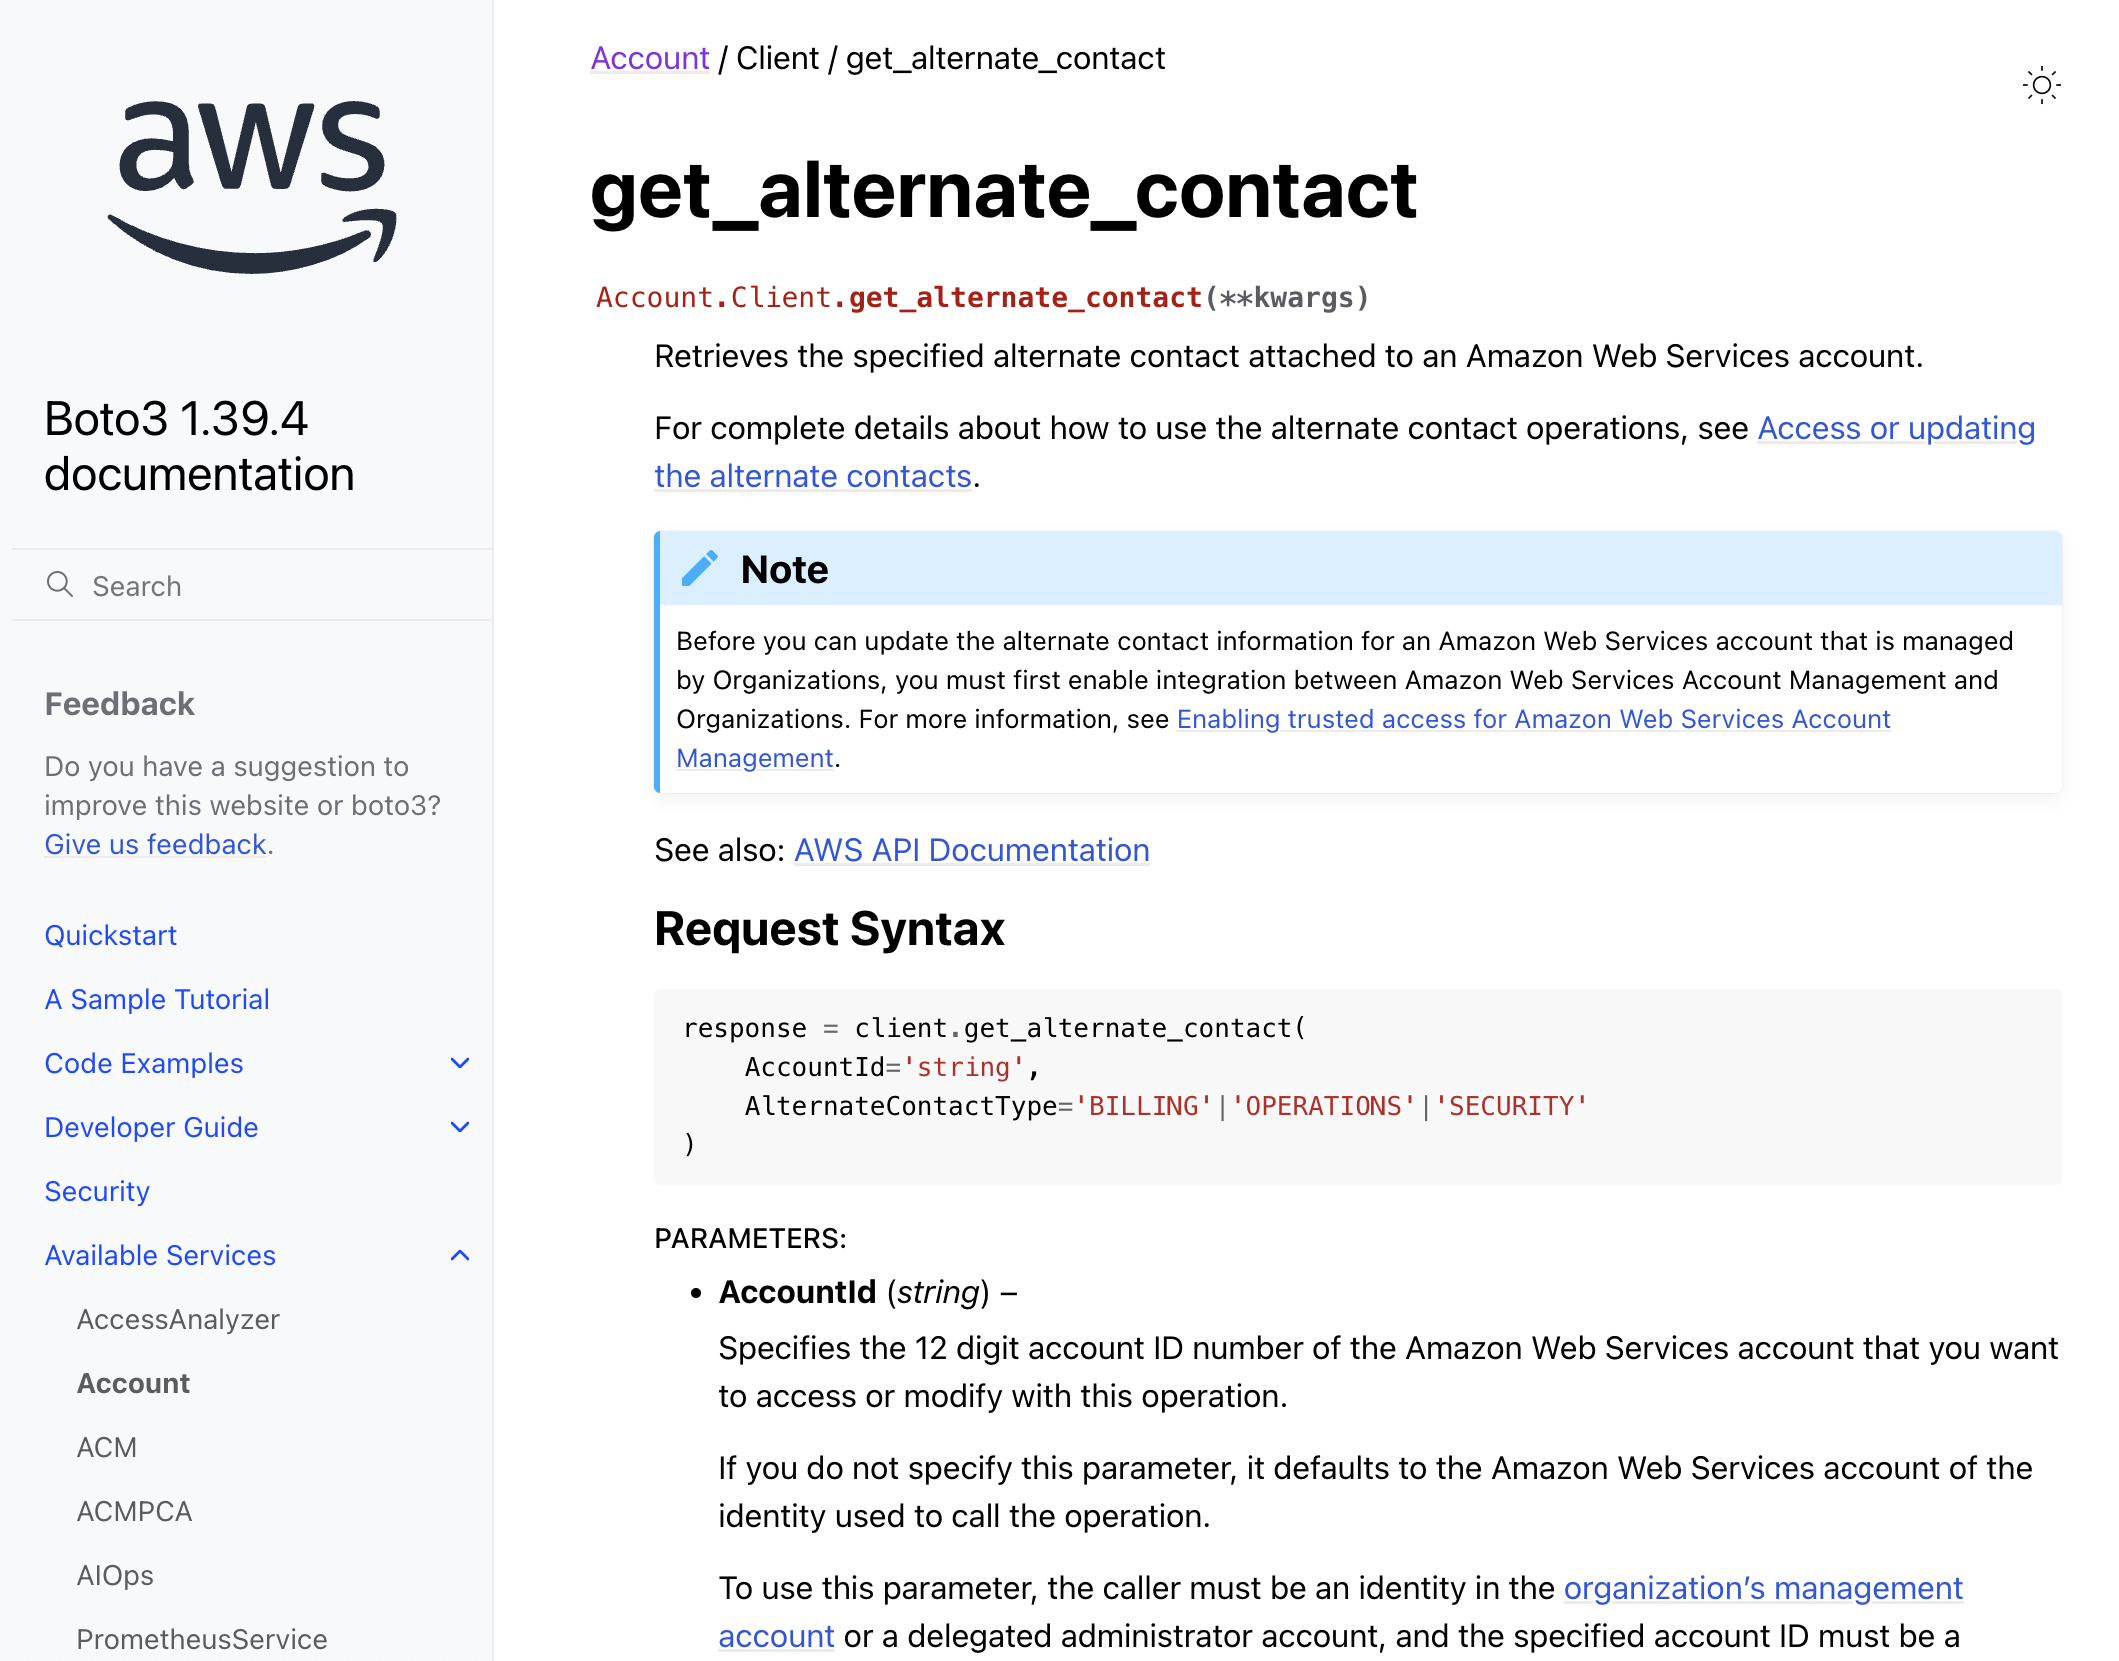
\includegraphics[width=\textwidth]{assets/boto3acc.png}
        \end{column}
    \end{columns}
\end{frame}

\begin{frame}{Suite di sonde}
    \framesubtitle{Elenco delle sonde sviluppate}
    \begin{columns}
        \begin{column}<1->{0.5\textwidth}
            \textbf{13} sonde sviluppate con \textbf{51} controlli
            \begin{itemize}
                \item \texttt{aws\_sqs}
                \item \texttt{aws\_inspector}
                \item \texttt{aws\_iam}
                \item \texttt{aws\_ec2}
                \item \texttt{aws\_s3}
                \item \texttt{aws\_account}
            \end{itemize}
        \end{column}
        \begin{column}<2->{0.5\textwidth}
            \begin{itemize}
                \item \texttt{aws\_config}
                \item \texttt{aws\_cloudtrail}
                \item  \texttt{aws\_efs}
                \item  \texttt{aws\_kms}
                \item  \texttt{aws\_rds}
                \item  \texttt{aws\_eks}
            \end{itemize}
        \end{column}
    \end{columns}
    \vspace{1em}
    \begin{itemize}
        \item <3-> \texttt{aws\_vulnerability}: aggregazione vulnerabilità da AWS Inspector (sonda fuori standard)
    \end{itemize}
\end{frame}

\begin{frame}{Moon Cloud}
    \framesubtitle{Piattaforma, funzionalità e architettura}
    \begin{columns}
        \begin{column}{0.4\textwidth}
            \begin{itemize}
                \item<1-> Esegue sonde di assurance su infrastrutture ICT
                \item<2-> Architettura basata su immagini Docker e CI/CD
                \item<3-> Dashboard per la gestione dei target, credenziali e risultati
            \end{itemize}
        \end{column}
        \begin{column}{0.6\textwidth}
            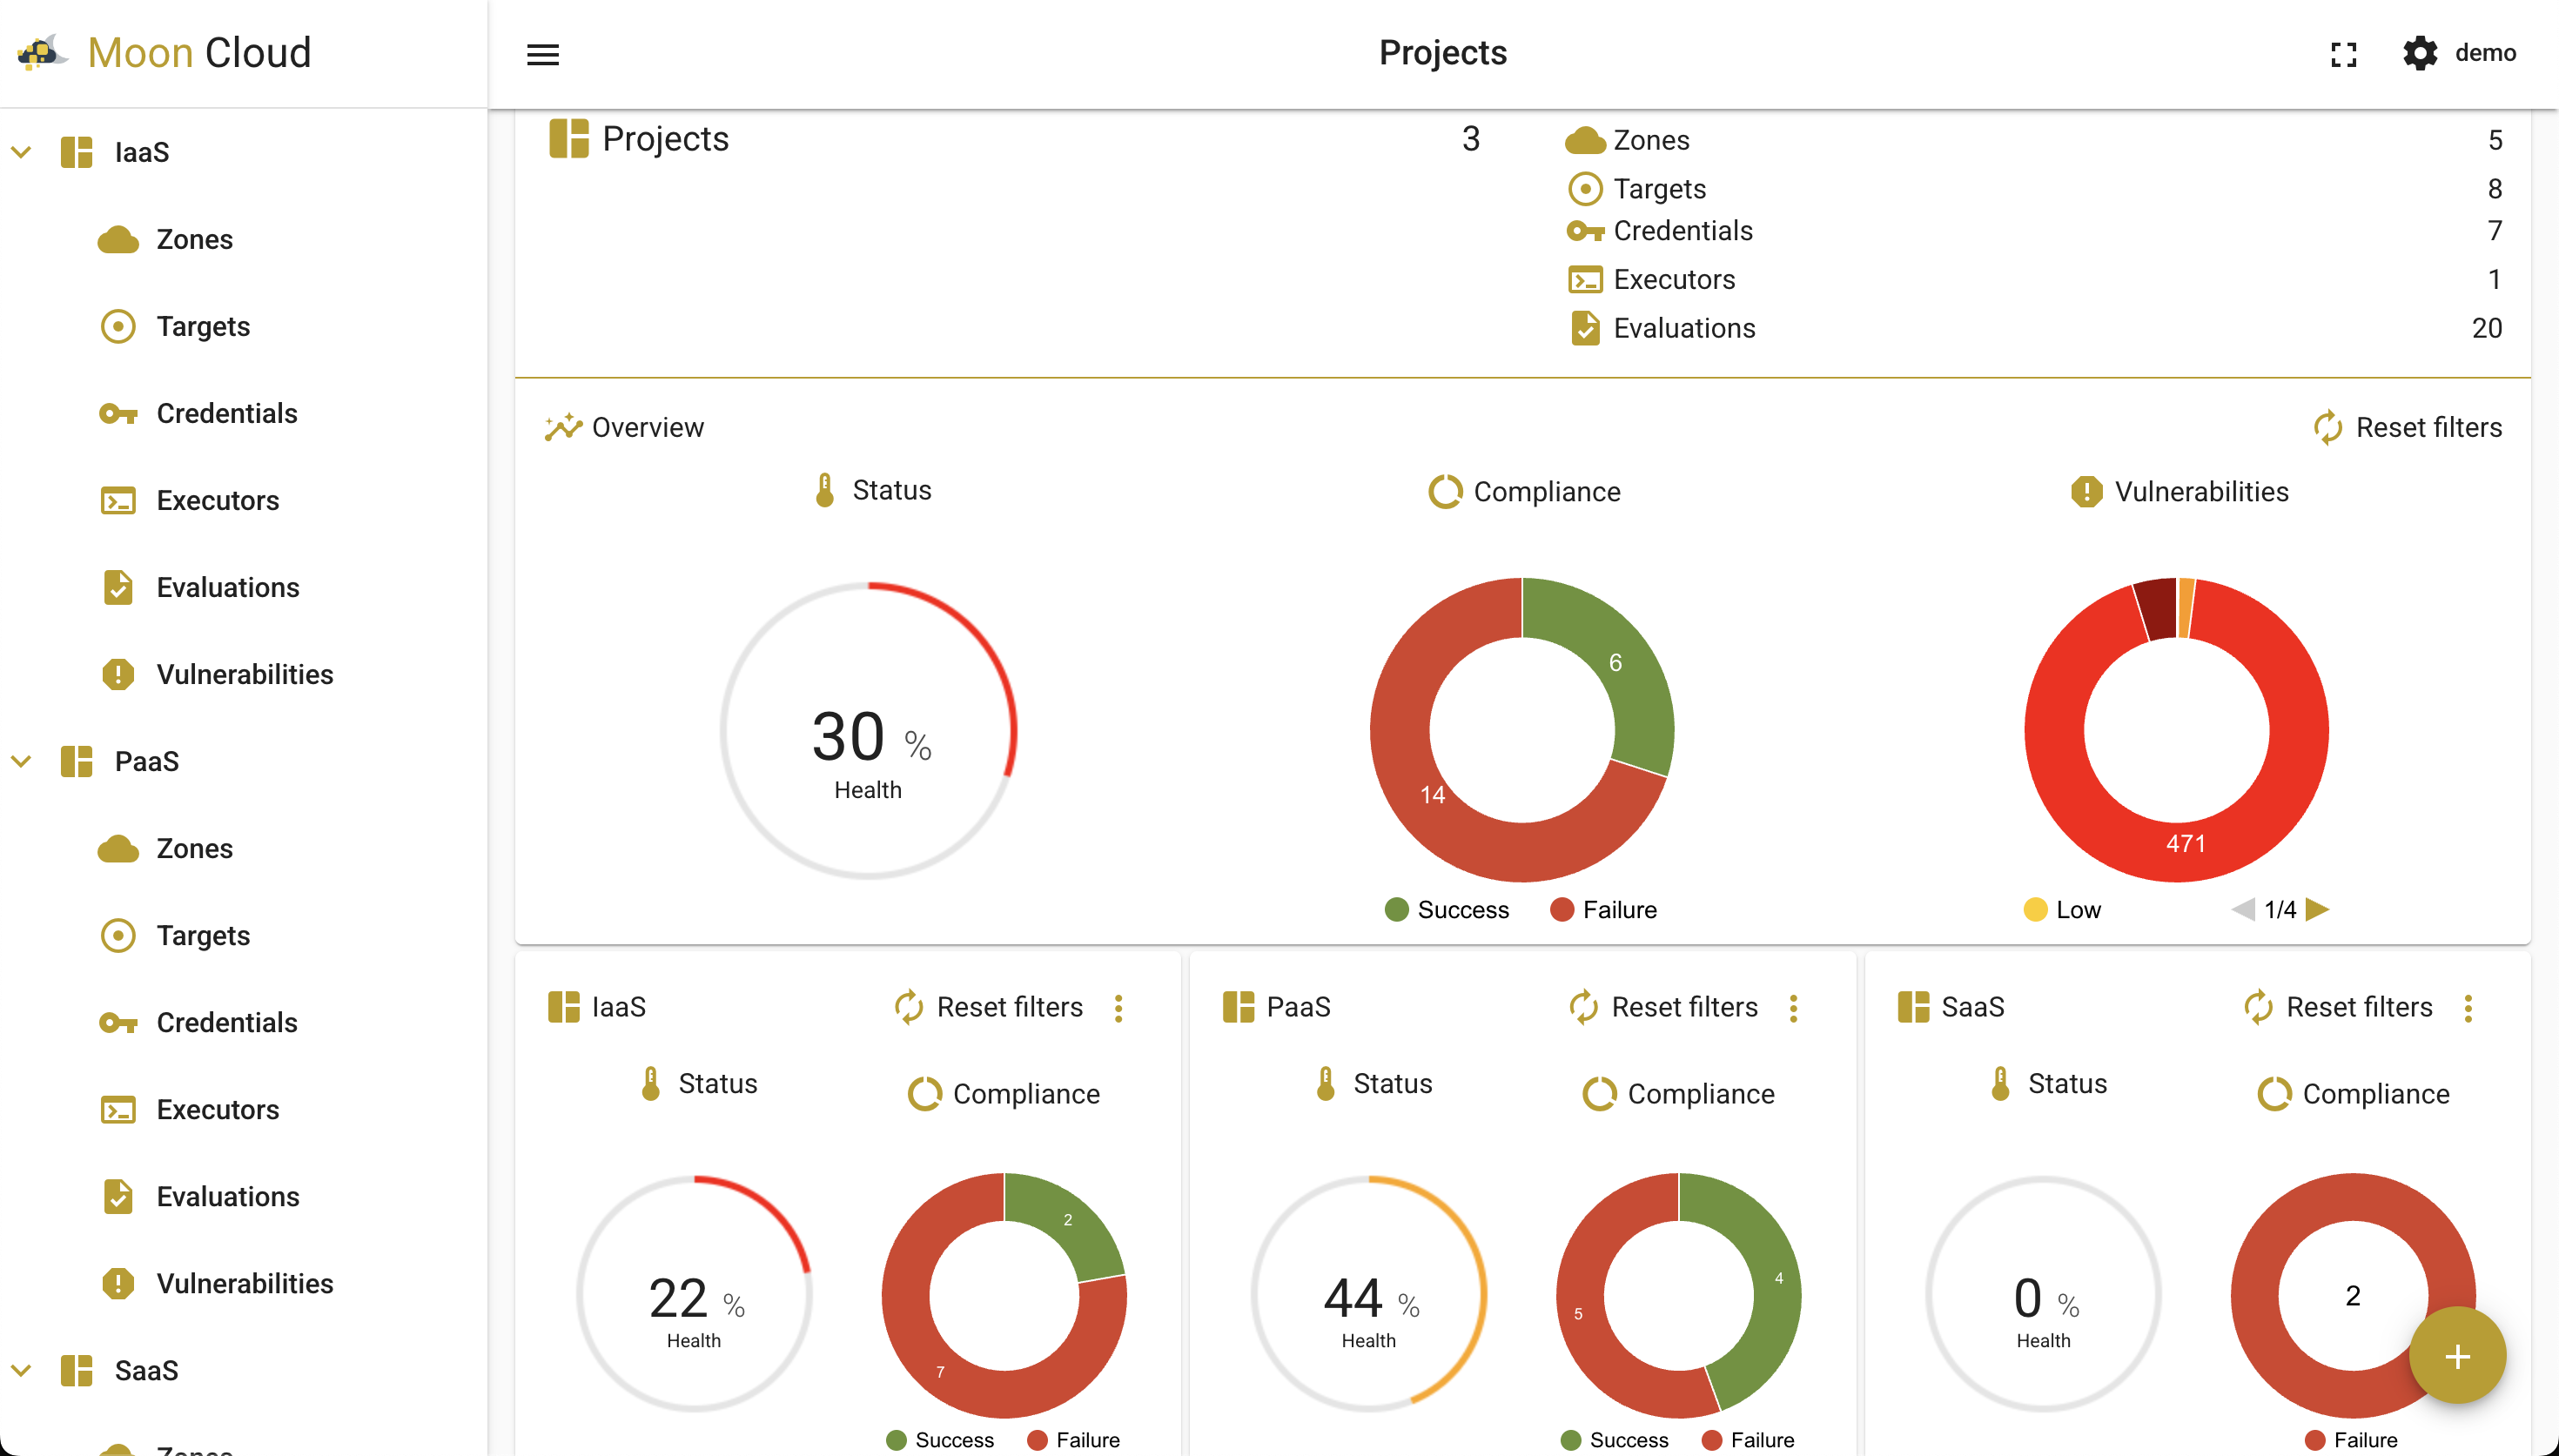
\includegraphics[width=\textwidth]{assets/dashboad.png}
        \end{column}
    \end{columns}
\end{frame}

\begin{frame}{Struttura di una sonda}
    \framesubtitle{Componenti per la creazione}
    \begin{columns}
        \begin{column}{0.6\textwidth}
            \begin{itemize}
                \item <1-> Struttura con \texttt{atoms} eseguiti in sequenza
                \item <2-> Modello a stati finiti: \textbf{forward} e \textbf{rollback}
                \item <3-> Output \emph{strutturato}
            \end{itemize}
        \end{column}
        \begin{column}<1->{0.4\textwidth}
            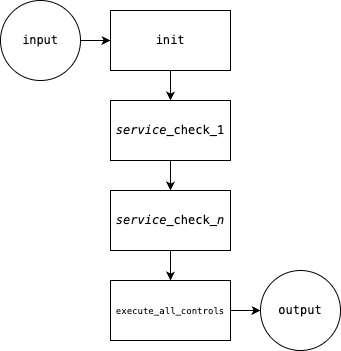
\includegraphics[width=\textwidth]{assets/flow.drawio.png}
        \end{column}
    \end{columns}
\end{frame}

\begin{frame}[fragile]{Esempio: \texttt{aws\_sqs}}
\framesubtitle{Controllo cifratura, tag e accesso pubblico}
\begin{itemize}
    \item<1-> Controlli relativi a crittografia, tagging, e policy pubbliche
    \item<2-> Integra scansione multiregione
    \item<3-> Ogni controllo è una funzione separata
\end{itemize}

\begin{onlyenv}<4->
\textbf{Snippet: gestione client multiregione e controllo SQS.1}
\begin{lstlisting}[style=statalepython, basicstyle=\scriptsize\ttfamily]
specific_regions = re.split(r'[,;\s]+', raw_regions) if raw_regions else []
for idx, region in enumerate(specific_regions[:6], start=1):
    self.clients[f'client_{idx}'] = boto3.client(...)
\end{lstlisting}
\end{onlyenv}
\begin{onlyenv}<5->
\begin{lstlisting}[style=statalepython, basicstyle=\scriptsize\ttfamily]
attr_response = client.get_queue_attributes(
    AttributeNames=['SqsManagedSseEnabled'],
    QueueUrl=queue_url
)
if attr_response.get('Attributes', {}).get('SqsManagedSseEnabled') == 'true':
    encrypted_queues.append(...)
else unencrypted_queues.append(...)
\end{lstlisting}
\end{onlyenv}
\end{frame}


\begin{frame}{\texttt{aws\_vulnerability}}
    \framesubtitle{Sonda per la gestione CVE}
    \begin{columns}
        \begin{column}{0.4\textwidth}
            \begin{itemize}
            \item<1-> Sonda che non aderisce a standard ma che elenca CVE trovate da AWS Inspector
            \item<2-> Analisi di Elastic Container Registry (\emph{ECR}), 
                Elastic Compute Cloud (\emph{EC2}) e \emph{Lambda} functions
            \item<3-> Consente una visione dinamica del rischio
        \end{itemize}
        \end{column}
        \begin{column}<4->{0.6\textwidth}
            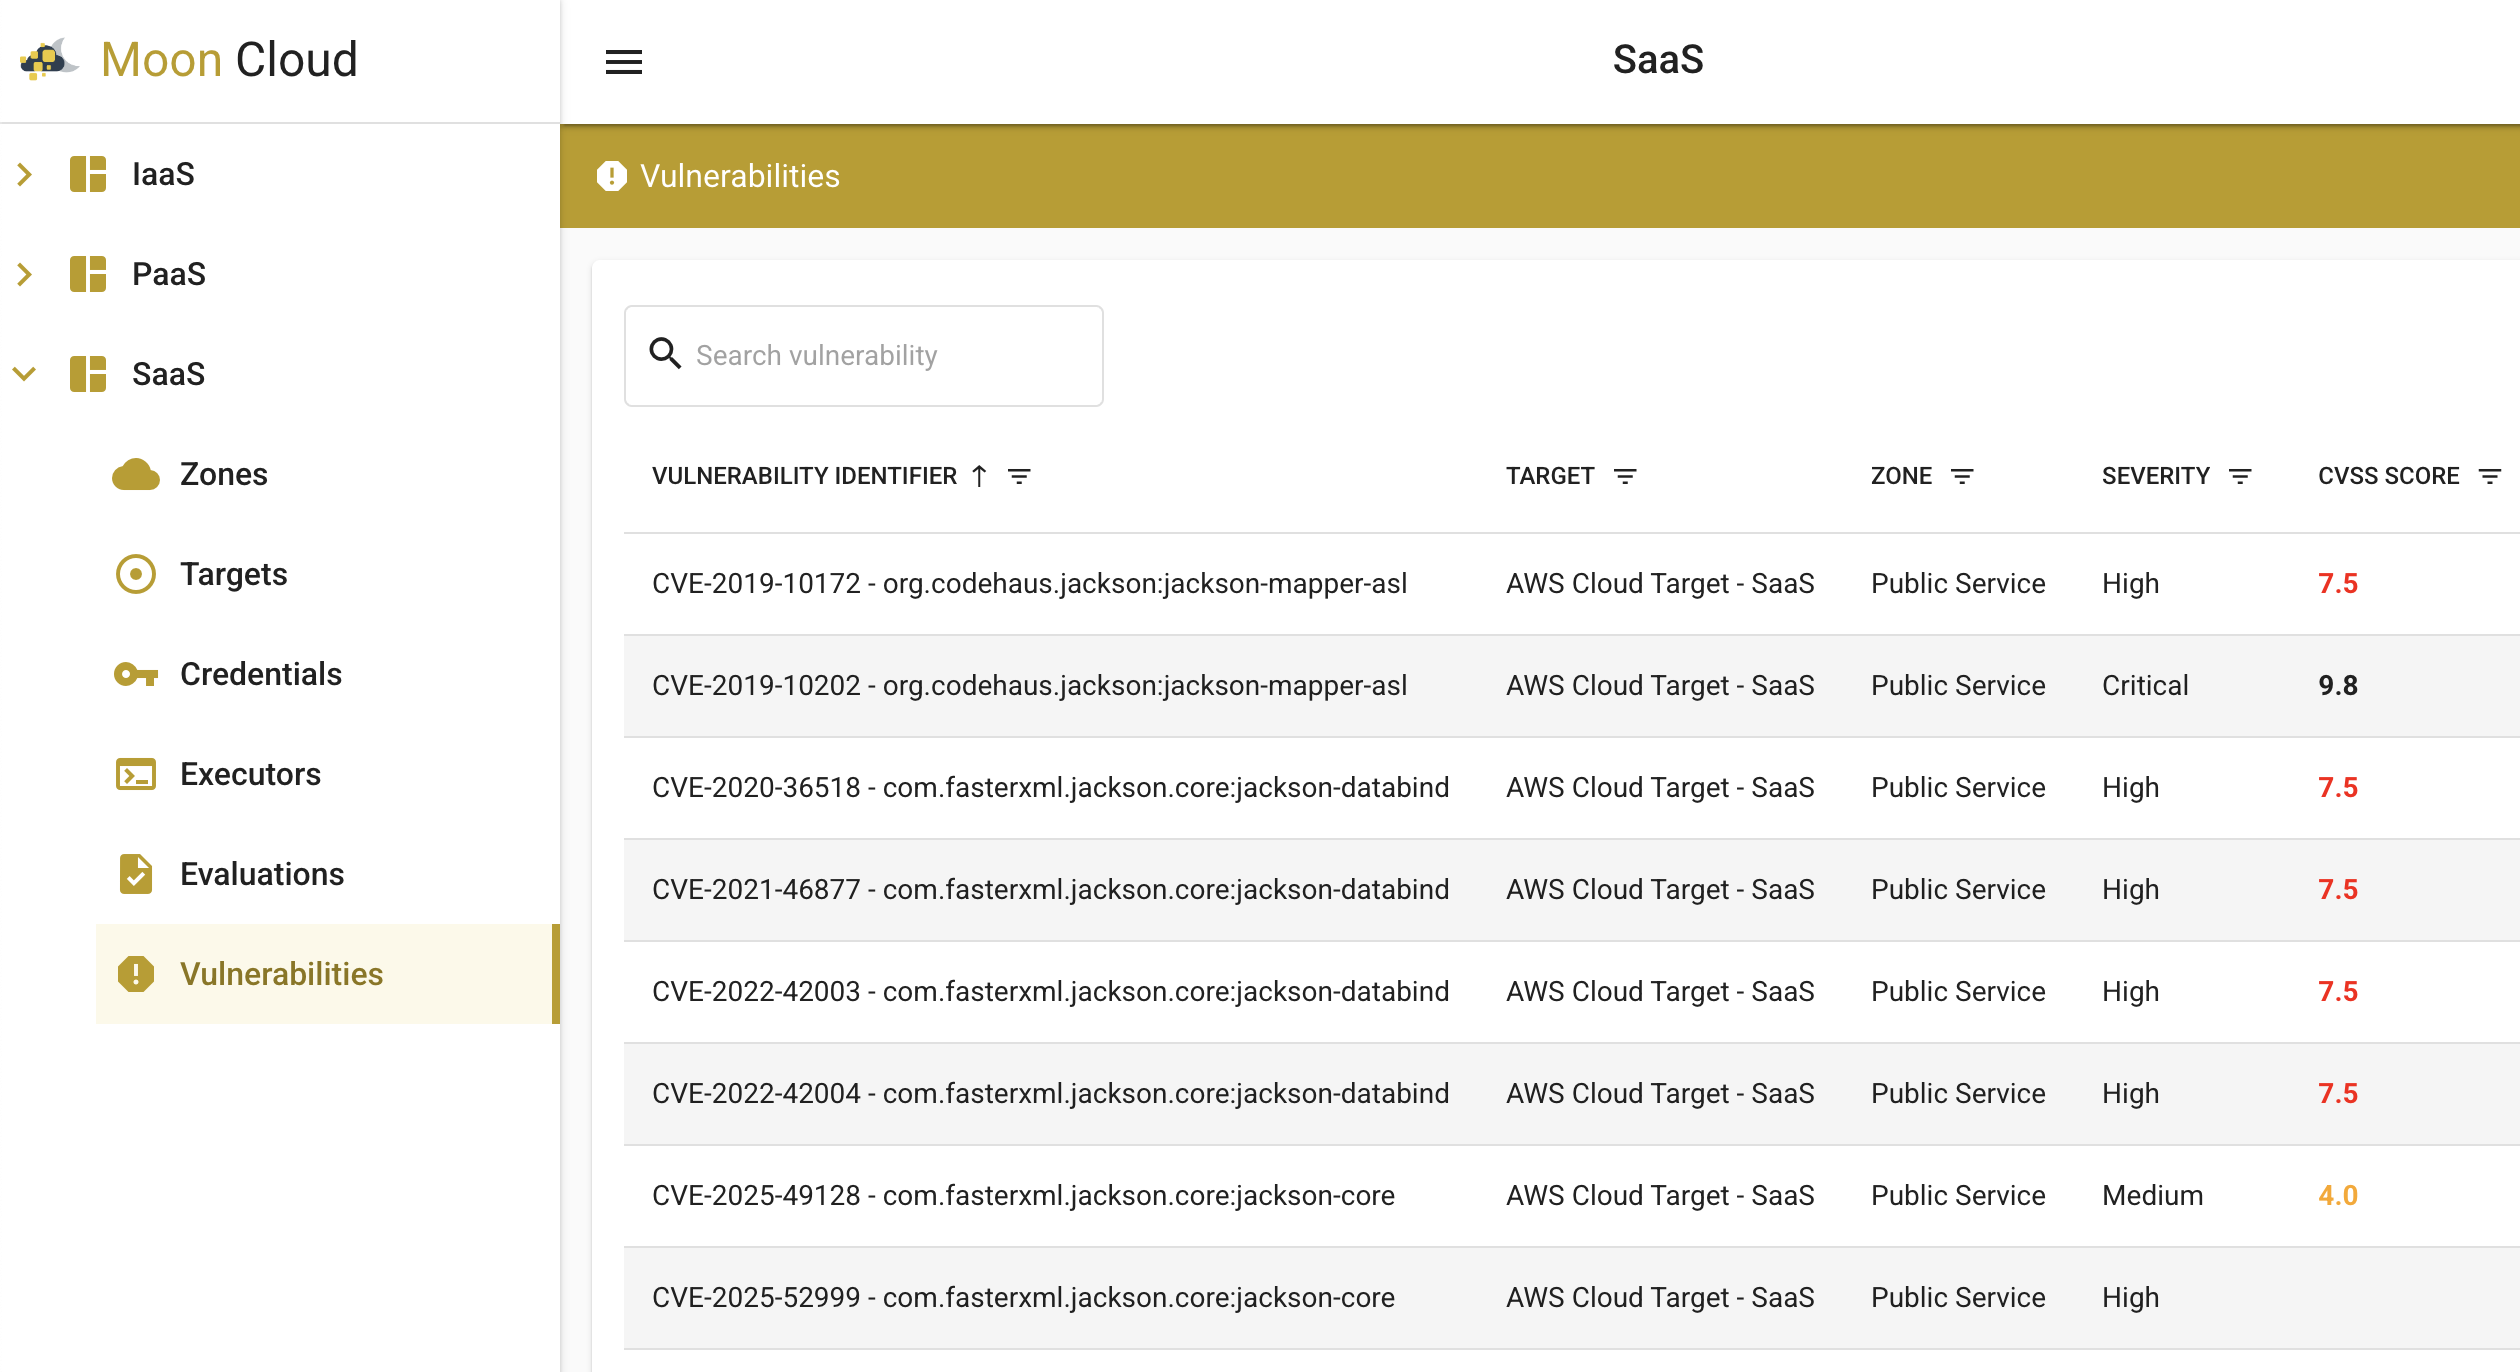
\includegraphics[width=\textwidth]{assets/cveiaas.png}
        \end{column}
    \end{columns}
\end{frame}

\begin{frame}{Deploy e output delle sonde}
    \framesubtitle{Esecuzione, integrazione e risultati}
    \begin{columns}
        \begin{column}<1->{0.4\textwidth}
            \textbf{Esecuzione e integrazione}
            \begin{itemize}
                \item Pipeline CI/CD su GitLab per ogni sonda
                \item Definizione rigorosa di \emph{Input} e \emph{Output}
                \item Definizione nel backend di Moon Cloud
                \item Integrazione nel frontend di Moon Cloud con \emph{template form}
            \end{itemize}
        \end{column}
        \begin{column}<2->{0.6\textwidth}
            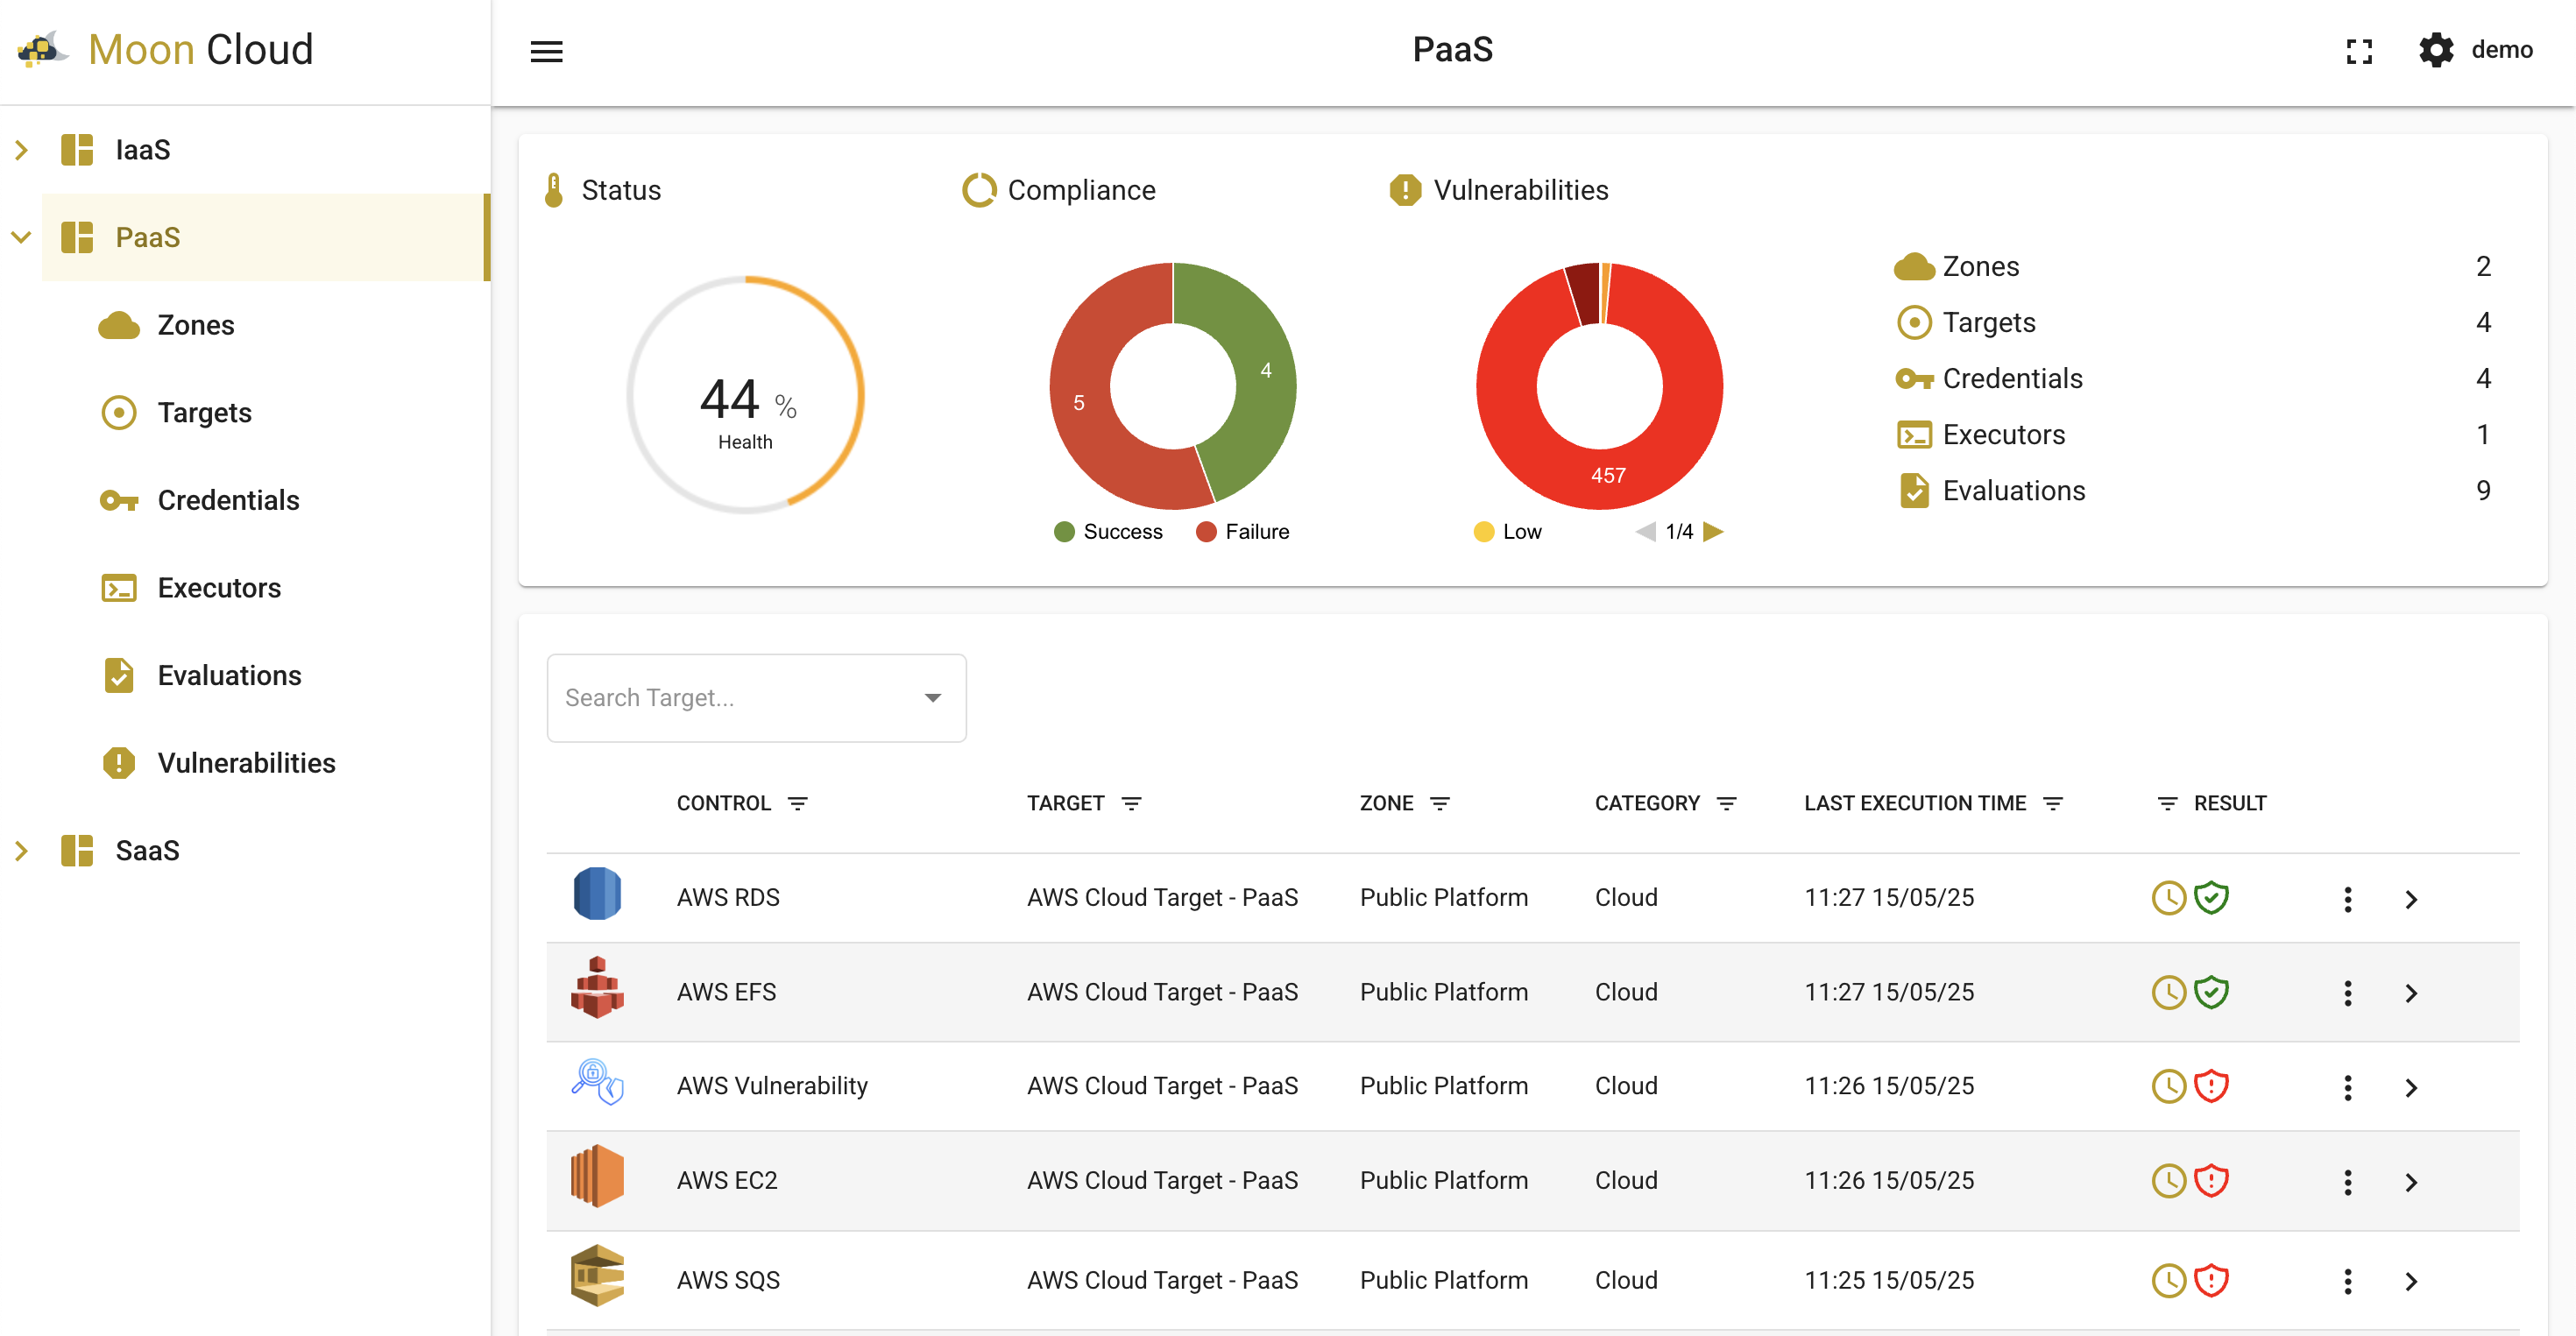
\includegraphics[width=\textwidth]{assets/paas.png}
        \end{column}
    \end{columns}
\end{frame}


\begin{frame}{Risultati ottenuti e sviluppi futuri}
    \framesubtitle{Riflessioni e prospettive}
    \begin{columns}
        \begin{column}<1->{0.5\textwidth}
            \textbf{Risultati ottenuti}
            \begin{itemize}
                \item Risultato numerico e descrittivo
                \item Sommario con percentuale di conformità
                \item Log dettagliato con eccezioni gestite
                \item Conformità a standard come CIS e NIST
            \end{itemize}
        \end{column}
        \begin{column}<2->{0.5\textwidth}
            \textbf{Sviluppi futuri}
            \begin{itemize}
                \item Estensione a nuovi benchmark e servizi AWS
                \item Apertura verso altri cloud provider
                \item Supporto multi regione
            \end{itemize}
        \end{column}
    \end{columns}
\end{frame}

% ==================///==================///==================///
% ==================/// END PRESENTATION
% ==================///==================///==================///

\backmatter
\end{document}